% Options for packages loaded elsewhere
\PassOptionsToPackage{unicode}{hyperref}
\PassOptionsToPackage{hyphens}{url}
%
\documentclass[
]{article}
\usepackage{amsmath,amssymb}
\usepackage{lmodern}
\usepackage{iftex}
\ifPDFTeX
  \usepackage[T1]{fontenc}
  \usepackage[utf8]{inputenc}
  \usepackage{textcomp} % provide euro and other symbols
\else % if luatex or xetex
  \usepackage{unicode-math}
  \defaultfontfeatures{Scale=MatchLowercase}
  \defaultfontfeatures[\rmfamily]{Ligatures=TeX,Scale=1}
\fi
% Use upquote if available, for straight quotes in verbatim environments
\IfFileExists{upquote.sty}{\usepackage{upquote}}{}
\IfFileExists{microtype.sty}{% use microtype if available
  \usepackage[]{microtype}
  \UseMicrotypeSet[protrusion]{basicmath} % disable protrusion for tt fonts
}{}
\makeatletter
\@ifundefined{KOMAClassName}{% if non-KOMA class
  \IfFileExists{parskip.sty}{%
    \usepackage{parskip}
  }{% else
    \setlength{\parindent}{0pt}
    \setlength{\parskip}{6pt plus 2pt minus 1pt}}
}{% if KOMA class
  \KOMAoptions{parskip=half}}
\makeatother
\usepackage{xcolor}
\usepackage[margin=1in]{geometry}
\usepackage{longtable,booktabs,array}
\usepackage{calc} % for calculating minipage widths
% Correct order of tables after \paragraph or \subparagraph
\usepackage{etoolbox}
\makeatletter
\patchcmd\longtable{\par}{\if@noskipsec\mbox{}\fi\par}{}{}
\makeatother
% Allow footnotes in longtable head/foot
\IfFileExists{footnotehyper.sty}{\usepackage{footnotehyper}}{\usepackage{footnote}}
\makesavenoteenv{longtable}
\usepackage{graphicx}
\makeatletter
\def\maxwidth{\ifdim\Gin@nat@width>\linewidth\linewidth\else\Gin@nat@width\fi}
\def\maxheight{\ifdim\Gin@nat@height>\textheight\textheight\else\Gin@nat@height\fi}
\makeatother
% Scale images if necessary, so that they will not overflow the page
% margins by default, and it is still possible to overwrite the defaults
% using explicit options in \includegraphics[width, height, ...]{}
\setkeys{Gin}{width=\maxwidth,height=\maxheight,keepaspectratio}
% Set default figure placement to htbp
\makeatletter
\def\fps@figure{htbp}
\makeatother
\setlength{\emergencystretch}{3em} % prevent overfull lines
\providecommand{\tightlist}{%
  \setlength{\itemsep}{0pt}\setlength{\parskip}{0pt}}
\setcounter{secnumdepth}{5}
\usepackage{booktabs}
\usepackage{longtable}
\usepackage{array}
\usepackage{multirow}
\usepackage{wrapfig}
\usepackage{float}
\usepackage{colortbl}
\usepackage{pdflscape}
\usepackage{tabu}
\usepackage{threeparttable}
\usepackage[normalem]{ulem}
\usepackage{makecell}
\usepackage{xcolor}
\usepackage{placeins}
\usepackage{booktabs}
\usepackage{longtable}
\usepackage{array}
\usepackage{multirow}
\usepackage{wrapfig}
\usepackage{float}
\usepackage{colortbl}
\usepackage{pdflscape}
\usepackage{tabu}
\usepackage{threeparttable}
\usepackage{threeparttablex}
\usepackage[normalem]{ulem}
\usepackage{makecell}
\usepackage{xcolor}
\ifLuaTeX
  \usepackage{selnolig}  % disable illegal ligatures
\fi
\IfFileExists{bookmark.sty}{\usepackage{bookmark}}{\usepackage{hyperref}}
\IfFileExists{xurl.sty}{\usepackage{xurl}}{} % add URL line breaks if available
\urlstyle{same} % disable monospaced font for URLs
\hypersetup{
  pdftitle={2023 Proposed CCFRP Otolith Collections},
  pdfauthor={Melissa H. Monk and Ellie Brauer},
  hidelinks,
  pdfcreator={LaTeX via pandoc}}

\title{2023 Proposed CCFRP Otolith Collections}
\author{Melissa H. Monk and Ellie Brauer}
\date{March 28, 2023}

\begin{document}
\maketitle

\hypertarget{first-pass-at-determining-2023-otolith-collections}{%
\section{First Pass at Determining 2023 Otolith Collections}\label{first-pass-at-determining-2023-otolith-collections}}

The following use only data from 2019, 2021 and 2022 from the reference areas. Drifts that did not see any of the target species are also excluded. I also excluded the following MPA locations, Farallons, Point Conception, Laguna Beach, Trinidad and ``BM'' (error?).

As a first pass, I looked at the total number of a given species by north and south
of Point Conception. I did this because we have been separating assessments at
Point Conception for most of the nearshore species, and species compositions and
fishing practices are fundamentally different in these two regions.\\
If there were fewer than 4 of a given species seen across the three years, I
excluded them from the collections analysis. I also removed yelloweye rockfish
and the olive or yellowtail rockfish category.

I then took the ratios of a
species within by CCFRP institution and scaled that to either a collection total
for each region of 50 samples (otoliths) or 70\% of the total. In an assessment model,
we usually exclude any age data with fewer than 30 samples per year.

I realize that we need to scale back some of the collections by programs, e.g., BML,
and also figure out if we should lingcod. The NWFSC is currently exploring
a comparison of lingcod otoliths reads with spine. Collection of spine is a bit more
difficult. There is also an interest in developing post-fillet back calculations
for lingcod. What I'd like to hear from each partner, is the maximum number of
otoliths you think you could possibly collect. We will also have staff available
to process fish (as long as COVID trends the right direction).

For species that are less common, otoliths can still be used to look at growth
curves, e.g.~copper and quillback this cycle.

I will clean up the tables below and look at a few other metrics including
available habitat in the reference sites for each university's site to make sure
we're scaling samples approporiately.

This document lives on my Github page and will allow us to reproduce these values
as a moving window going forward, and also adjust according to assessment
prioritization. The Council will decide a preliminary assessments for the odd year
in the prior even year, with final decisions coming in June. That should give us
time to adjust these numbers for special collections.

We also have an interest in fin clips, especially for vermilion/sunsets and also
blue/deacons.

\newpage

\begin{table}

\caption{\label{tab:anghrs}Total angler hours by institution summed across 2019, 2021, 2022.}
\centering
\begin{tabular}[t]{rrrrrrr}
\toprule
YEAR & BML & Cal Poly & HSU & MLML & SIO & UCSB\\
\midrule
\cellcolor{gray!6}{2019} & \cellcolor{gray!6}{193} & \cellcolor{gray!6}{172} & \cellcolor{gray!6}{66} & \cellcolor{gray!6}{187} & \cellcolor{gray!6}{97} & \cellcolor{gray!6}{110}\\
2021 & 110 & 112 & 65 & 161 & 39 & 151\\
\cellcolor{gray!6}{2022} & \cellcolor{gray!6}{97} & \cellcolor{gray!6}{139} & \cellcolor{gray!6}{71} & \cellcolor{gray!6}{207} & \cellcolor{gray!6}{143} & \cellcolor{gray!6}{170}\\
\bottomrule
\end{tabular}
\end{table}

\begin{table}

\caption{\label{tab:effort2022}Total effort in 2022}
\centering
\begin{tabular}[t]{lrl}
\toprule
Monitoring.Group & Total\_AnglerHours & Percent\_Effort\\
\midrule
\cellcolor{gray!6}{BML} & \cellcolor{gray!6}{97} & \cellcolor{gray!6}{12\%}\\
Cal Poly & 139 & 17\%\\
\cellcolor{gray!6}{HSU} & \cellcolor{gray!6}{71} & \cellcolor{gray!6}{9\%}\\
MLML & 207 & 25\%\\
\cellcolor{gray!6}{SIO} & \cellcolor{gray!6}{143} & \cellcolor{gray!6}{17\%}\\
\addlinespace
UCSB & 170 & 21\%\\
\bottomrule
\end{tabular}
\end{table}

\begin{table}

\caption{\label{tab:effort2019}Total effort in 2019}
\centering
\begin{tabular}[t]{lrl}
\toprule
Monitoring.Group & Total\_AnglerHours & Percent\_Effort\\
\midrule
BML & 193 & 23\%\\
Cal Poly & 172 & 21\%\\
HSU & 66 & 8\%\\
MLML & 187 & 23\%\\
SIO & 97 & 12\%\\
\addlinespace
UCSB & 110 & 13\%\\
\bottomrule
\end{tabular}
\end{table}

\begin{table}

\caption{\label{tab:collections}Suggested otolith collections for 2023 CCFRP by species and CCFRP partner}
\centering
\begin{tabular}[t]{lrrrrrrr}
\toprule
Common.Name & BML & HSU & MLML & Cal Poly & UCSB & SIO & Total\\
\midrule
\cellcolor{gray!6}{Black Rockfish} & \cellcolor{gray!6}{10} & \cellcolor{gray!6}{11} & \cellcolor{gray!6}{30} & \cellcolor{gray!6}{0} & \cellcolor{gray!6}{0} & \cellcolor{gray!6}{0} & \cellcolor{gray!6}{51}\\
Black-and-Yellow Rockfish & 11 & 0 & 7 & 0 & 0 & 0 & 18\\
\cellcolor{gray!6}{Blue Rockfish} & \cellcolor{gray!6}{10} & \cellcolor{gray!6}{3} & \cellcolor{gray!6}{23} & \cellcolor{gray!6}{15} & \cellcolor{gray!6}{50} & \cellcolor{gray!6}{0} & \cellcolor{gray!6}{101}\\
Brown Rockfish & 31 & 0 & 20 & 0 & 5 & 0 & 56\\
\cellcolor{gray!6}{Calico Rockfish} & \cellcolor{gray!6}{0} & \cellcolor{gray!6}{0} & \cellcolor{gray!6}{0} & \cellcolor{gray!6}{4} & \cellcolor{gray!6}{0} & \cellcolor{gray!6}{16} & \cellcolor{gray!6}{20}\\
\addlinespace
Canary Rockfish & 28 & 20 & 3 & 0 & 0 & 0 & 51\\
\cellcolor{gray!6}{China Rockfish} & \cellcolor{gray!6}{19} & \cellcolor{gray!6}{9} & \cellcolor{gray!6}{23} & \cellcolor{gray!6}{0} & \cellcolor{gray!6}{0} & \cellcolor{gray!6}{0} & \cellcolor{gray!6}{51}\\
Copper Rockfish & 21 & 15 & 6 & 9 & 50 & 0 & 101\\
\cellcolor{gray!6}{Deacon Rockfish} & \cellcolor{gray!6}{38} & \cellcolor{gray!6}{13} & \cellcolor{gray!6}{1} & \cellcolor{gray!6}{0} & \cellcolor{gray!6}{0} & \cellcolor{gray!6}{0} & \cellcolor{gray!6}{52}\\
Gopher Rockfish & 10 & 1 & 23 & 18 & 33 & 5 & 90\\
\addlinespace
\cellcolor{gray!6}{Kelp Rockfish} & \cellcolor{gray!6}{0} & \cellcolor{gray!6}{0} & \cellcolor{gray!6}{11} & \cellcolor{gray!6}{17} & \cellcolor{gray!6}{7} & \cellcolor{gray!6}{5} & \cellcolor{gray!6}{40}\\
Olive Rockfish & 7 & 3 & 21 & 21 & 4 & 5 & 61\\
\cellcolor{gray!6}{Quillback Rockfish} & \cellcolor{gray!6}{4} & \cellcolor{gray!6}{13} & \cellcolor{gray!6}{0} & \cellcolor{gray!6}{0} & \cellcolor{gray!6}{0} & \cellcolor{gray!6}{0} & \cellcolor{gray!6}{17}\\
Rosy Rockfish & 13 & 17 & 14 & 7 & 8 & 5 & 64\\
\cellcolor{gray!6}{Treefish} & \cellcolor{gray!6}{0} & \cellcolor{gray!6}{0} & \cellcolor{gray!6}{4} & \cellcolor{gray!6}{7} & \cellcolor{gray!6}{19} & \cellcolor{gray!6}{9} & \cellcolor{gray!6}{39}\\
\addlinespace
Vermilion Rockfish & 11 & 9 & 14 & 18 & 18 & 14 & 84\\
\cellcolor{gray!6}{Yellowtail Rockfish} & \cellcolor{gray!6}{20} & \cellcolor{gray!6}{14} & \cellcolor{gray!6}{12} & \cellcolor{gray!6}{6} & \cellcolor{gray!6}{0} & \cellcolor{gray!6}{0} & \cellcolor{gray!6}{52}\\
Honeycomb Rockfish & 0 & 0 & 0 & 0 & 0 & 45 & 45\\
\cellcolor{gray!6}{Starry Rockfish} & \cellcolor{gray!6}{0} & \cellcolor{gray!6}{0} & \cellcolor{gray!6}{0} & \cellcolor{gray!6}{0} & \cellcolor{gray!6}{4} & \cellcolor{gray!6}{0} & \cellcolor{gray!6}{4}\\
\bottomrule
\end{tabular}
\end{table}

\begin{table}

\caption{\label{tab:partnernumbers}Number of structures to collect by partner for 2023 CCFRP}
\centering
\begin{tabular}[t]{lr}
\toprule
Monitoring.Group & total\_fish\_for\_otoliths\\
\midrule
SIO & 104\\
UCSB & 198\\
BML & 233\\
Cal Poly & 122\\
HSU & 128\\
\addlinespace
MLML & 212\\
\bottomrule
\end{tabular}
\end{table}

\FloatBarrier

\clearpage
\newpage

\begin{longtable}[t]{llrlrr}
\caption{\label{tab:specieslong}Longer table with raw data}\\
\toprule
Common.Name & Monitoring.Group & YEAR & Region & total\_fish & avg\_annual\_cpue\\
\midrule
\endfirsthead
\caption[]{\label{tab:specieslong}Longer table with raw data \textit{(continued)}}\\
\toprule
Common.Name & Monitoring.Group & YEAR & Region & total\_fish & avg\_annual\_cpue\\
\midrule
\endhead

\endfoot
\bottomrule
\endlastfoot
\cellcolor{gray!6}{Black Rockfish} & \cellcolor{gray!6}{BML} & \cellcolor{gray!6}{2019} & \cellcolor{gray!6}{North} & \cellcolor{gray!6}{203} & \cellcolor{gray!6}{2.2099078}\\
Black Rockfish & BML & 2021 & North & 171 & 2.4034809\\
\cellcolor{gray!6}{Black Rockfish} & \cellcolor{gray!6}{BML} & \cellcolor{gray!6}{2022} & \cellcolor{gray!6}{North} & \cellcolor{gray!6}{22} & \cellcolor{gray!6}{2.0995808}\\
Black Rockfish & Cal Poly & 2019 & Central & 4 & 1.3318535\\
\cellcolor{gray!6}{Black Rockfish} & \cellcolor{gray!6}{Cal Poly} & \cellcolor{gray!6}{2021} & \cellcolor{gray!6}{Central} & \cellcolor{gray!6}{1} & \cellcolor{gray!6}{0.5000000}\\
\addlinespace
Black Rockfish & Cal Poly & 2022 & Central & 4 & 0.4850820\\
\cellcolor{gray!6}{Black Rockfish} & \cellcolor{gray!6}{HSU} & \cellcolor{gray!6}{2019} & \cellcolor{gray!6}{North} & \cellcolor{gray!6}{77} & \cellcolor{gray!6}{4.2079416}\\
Black Rockfish & HSU & 2021 & North & 202 & 6.4680716\\
\cellcolor{gray!6}{Black Rockfish} & \cellcolor{gray!6}{HSU} & \cellcolor{gray!6}{2022} & \cellcolor{gray!6}{North} & \cellcolor{gray!6}{190} & \cellcolor{gray!6}{4.5540686}\\
Black Rockfish & MLML & 2019 & Central & 389 & 4.2255708\\
\addlinespace
\cellcolor{gray!6}{Black Rockfish} & \cellcolor{gray!6}{MLML} & \cellcolor{gray!6}{2021} & \cellcolor{gray!6}{Central} & \cellcolor{gray!6}{477} & \cellcolor{gray!6}{5.9384010}\\
Black Rockfish & MLML & 2022 & Central & 422 & 3.8762804\\
\cellcolor{gray!6}{Black Rockfish} & \cellcolor{gray!6}{UCSB} & \cellcolor{gray!6}{2021} & \cellcolor{gray!6}{South} & \cellcolor{gray!6}{2} & \cellcolor{gray!6}{0.7692308}\\
Black-and-Yellow Rockfish & BML & 2019 & North & 5 & 1.6666667\\
\cellcolor{gray!6}{Black-and-Yellow Rockfish} & \cellcolor{gray!6}{BML} & \cellcolor{gray!6}{2021} & \cellcolor{gray!6}{North} & \cellcolor{gray!6}{21} & \cellcolor{gray!6}{2.8042328}\\
\addlinespace
Black-and-Yellow Rockfish & BML & 2022 & North & 19 & 1.6711243\\
\cellcolor{gray!6}{Black-and-Yellow Rockfish} & \cellcolor{gray!6}{Cal Poly} & \cellcolor{gray!6}{2021} & \cellcolor{gray!6}{Central} & \cellcolor{gray!6}{1} & \cellcolor{gray!6}{0.6666667}\\
Black-and-Yellow Rockfish & Cal Poly & 2022 & Central & 1 & 0.5682715\\
\cellcolor{gray!6}{Black-and-Yellow Rockfish} & \cellcolor{gray!6}{MLML} & \cellcolor{gray!6}{2019} & \cellcolor{gray!6}{Central} & \cellcolor{gray!6}{3} & \cellcolor{gray!6}{0.5980114}\\
Black-and-Yellow Rockfish & MLML & 2021 & Central & 21 & 2.8024699\\
\addlinespace
\cellcolor{gray!6}{Black-and-Yellow Rockfish} & \cellcolor{gray!6}{MLML} & \cellcolor{gray!6}{2022} & \cellcolor{gray!6}{Central} & \cellcolor{gray!6}{2} & \cellcolor{gray!6}{0.3329638}\\
Black-and-Yellow Rockfish & UCSB & 2019 & South & 2 & 0.3076923\\
\cellcolor{gray!6}{Black-and-Yellow Rockfish} & \cellcolor{gray!6}{UCSB} & \cellcolor{gray!6}{2021} & \cellcolor{gray!6}{South} & \cellcolor{gray!6}{1} & \cellcolor{gray!6}{0.4615385}\\
Blue Rockfish & BML & 2019 & North & 476 & 4.1525805\\
\cellcolor{gray!6}{Blue Rockfish} & \cellcolor{gray!6}{BML} & \cellcolor{gray!6}{2021} & \cellcolor{gray!6}{North} & \cellcolor{gray!6}{344} & \cellcolor{gray!6}{3.9604359}\\
\addlinespace
Blue Rockfish & BML & 2022 & North & 144 & 3.5162611\\
\cellcolor{gray!6}{Blue Rockfish} & \cellcolor{gray!6}{Cal Poly} & \cellcolor{gray!6}{2019} & \cellcolor{gray!6}{Central} & \cellcolor{gray!6}{977} & \cellcolor{gray!6}{8.2070904}\\
Blue Rockfish & Cal Poly & 2021 & Central & 396 & 6.3859919\\
\cellcolor{gray!6}{Blue Rockfish} & \cellcolor{gray!6}{Cal Poly} & \cellcolor{gray!6}{2022} & \cellcolor{gray!6}{Central} & \cellcolor{gray!6}{97} & \cellcolor{gray!6}{1.8102338}\\
Blue Rockfish & HSU & 2019 & North & 54 & 2.5111033\\
\addlinespace
\cellcolor{gray!6}{Blue Rockfish} & \cellcolor{gray!6}{HSU} & \cellcolor{gray!6}{2021} & \cellcolor{gray!6}{North} & \cellcolor{gray!6}{114} & \cellcolor{gray!6}{6.3118302}\\
Blue Rockfish & HSU & 2022 & North & 114 & 4.4491360\\
\cellcolor{gray!6}{Blue Rockfish} & \cellcolor{gray!6}{MLML} & \cellcolor{gray!6}{2019} & \cellcolor{gray!6}{Central} & \cellcolor{gray!6}{1429} & \cellcolor{gray!6}{7.9574113}\\
Blue Rockfish & MLML & 2021 & Central & 473 & 3.3025650\\
\cellcolor{gray!6}{Blue Rockfish} & \cellcolor{gray!6}{MLML} & \cellcolor{gray!6}{2022} & \cellcolor{gray!6}{Central} & \cellcolor{gray!6}{368} & \cellcolor{gray!6}{2.3472667}\\
\addlinespace
Blue Rockfish & UCSB & 2019 & South & 221 & 3.4026773\\
\cellcolor{gray!6}{Blue Rockfish} & \cellcolor{gray!6}{UCSB} & \cellcolor{gray!6}{2021} & \cellcolor{gray!6}{South} & \cellcolor{gray!6}{222} & \cellcolor{gray!6}{2.8199352}\\
Blue Rockfish & UCSB & 2022 & South & 187 & 1.7926313\\
\cellcolor{gray!6}{Bocaccio} & \cellcolor{gray!6}{MLML} & \cellcolor{gray!6}{2022} & \cellcolor{gray!6}{Central} & \cellcolor{gray!6}{2} & \cellcolor{gray!6}{0.3493891}\\
Brown Rockfish & BML & 2019 & North & 61 & 1.8121751\\
\addlinespace
\cellcolor{gray!6}{Brown Rockfish} & \cellcolor{gray!6}{BML} & \cellcolor{gray!6}{2021} & \cellcolor{gray!6}{North} & \cellcolor{gray!6}{56} & \cellcolor{gray!6}{1.4569106}\\
Brown Rockfish & BML & 2022 & North & 56 & 1.4372981\\
\cellcolor{gray!6}{Brown Rockfish} & \cellcolor{gray!6}{Cal Poly} & \cellcolor{gray!6}{2019} & \cellcolor{gray!6}{Central} & \cellcolor{gray!6}{2} & \cellcolor{gray!6}{0.6645613}\\
Brown Rockfish & HSU & 2019 & North & 2 & 2.0000000\\
\cellcolor{gray!6}{Brown Rockfish} & \cellcolor{gray!6}{HSU} & \cellcolor{gray!6}{2022} & \cellcolor{gray!6}{North} & \cellcolor{gray!6}{1} & \cellcolor{gray!6}{0.7500000}\\
\addlinespace
Brown Rockfish & MLML & 2019 & Central & 19 & 1.0373537\\
\cellcolor{gray!6}{Brown Rockfish} & \cellcolor{gray!6}{MLML} & \cellcolor{gray!6}{2021} & \cellcolor{gray!6}{Central} & \cellcolor{gray!6}{29} & \cellcolor{gray!6}{1.0903884}\\
Brown Rockfish & MLML & 2022 & Central & 64 & 1.4731689\\
\cellcolor{gray!6}{Brown Rockfish} & \cellcolor{gray!6}{SIO} & \cellcolor{gray!6}{2019} & \cellcolor{gray!6}{South} & \cellcolor{gray!6}{1} & \cellcolor{gray!6}{0.3076923}\\
Brown Rockfish & SIO & 2021 & South & 3 & 0.6349206\\
\addlinespace
\cellcolor{gray!6}{Brown Rockfish} & \cellcolor{gray!6}{SIO} & \cellcolor{gray!6}{2022} & \cellcolor{gray!6}{South} & \cellcolor{gray!6}{6} & \cellcolor{gray!6}{0.4095238}\\
Brown Rockfish & UCSB & 2019 & South & 13 & 1.4358974\\
\cellcolor{gray!6}{Brown Rockfish} & \cellcolor{gray!6}{UCSB} & \cellcolor{gray!6}{2021} & \cellcolor{gray!6}{South} & \cellcolor{gray!6}{1} & \cellcolor{gray!6}{0.4395604}\\
Brown Rockfish & UCSB & 2022 & South & 6 & 0.7012987\\
\cellcolor{gray!6}{Calico Rockfish} & \cellcolor{gray!6}{Cal Poly} & \cellcolor{gray!6}{2019} & \cellcolor{gray!6}{Central} & \cellcolor{gray!6}{1} & \cellcolor{gray!6}{0.3322259}\\
\addlinespace
Calico Rockfish & Cal Poly & 2021 & Central & 7 & 0.6702619\\
\cellcolor{gray!6}{Calico Rockfish} & \cellcolor{gray!6}{Cal Poly} & \cellcolor{gray!6}{2022} & \cellcolor{gray!6}{Central} & \cellcolor{gray!6}{6} & \cellcolor{gray!6}{0.6760562}\\
Calico Rockfish & SIO & 2019 & South & 26 & 1.0522509\\
\cellcolor{gray!6}{Calico Rockfish} & \cellcolor{gray!6}{SIO} & \cellcolor{gray!6}{2021} & \cellcolor{gray!6}{South} & \cellcolor{gray!6}{12} & \cellcolor{gray!6}{0.8075758}\\
Calico Rockfish & SIO & 2022 & South & 27 & 0.5230159\\
\addlinespace
\cellcolor{gray!6}{Canary Rockfish} & \cellcolor{gray!6}{BML} & \cellcolor{gray!6}{2019} & \cellcolor{gray!6}{North} & \cellcolor{gray!6}{57} & \cellcolor{gray!6}{1.5591921}\\
Canary Rockfish & BML & 2021 & North & 109 & 4.3635913\\
\cellcolor{gray!6}{Canary Rockfish} & \cellcolor{gray!6}{BML} & \cellcolor{gray!6}{2022} & \cellcolor{gray!6}{North} & \cellcolor{gray!6}{64} & \cellcolor{gray!6}{1.7360041}\\
Canary Rockfish & HSU & 2019 & North & 62 & 2.4968405\\
\cellcolor{gray!6}{Canary Rockfish} & \cellcolor{gray!6}{HSU} & \cellcolor{gray!6}{2021} & \cellcolor{gray!6}{North} & \cellcolor{gray!6}{57} & \cellcolor{gray!6}{2.3458428}\\
\addlinespace
Canary Rockfish & HSU & 2022 & North & 48 & 1.7236162\\
\cellcolor{gray!6}{Canary Rockfish} & \cellcolor{gray!6}{MLML} & \cellcolor{gray!6}{2019} & \cellcolor{gray!6}{Central} & \cellcolor{gray!6}{7} & \cellcolor{gray!6}{0.4694076}\\
Canary Rockfish & MLML & 2021 & Central & 6 & 1.1709987\\
\cellcolor{gray!6}{Canary Rockfish} & \cellcolor{gray!6}{MLML} & \cellcolor{gray!6}{2022} & \cellcolor{gray!6}{Central} & \cellcolor{gray!6}{11} & \cellcolor{gray!6}{0.7282766}\\
China Rockfish & BML & 2019 & North & 68 & 0.7586641\\
\addlinespace
\cellcolor{gray!6}{China Rockfish} & \cellcolor{gray!6}{BML} & \cellcolor{gray!6}{2021} & \cellcolor{gray!6}{North} & \cellcolor{gray!6}{60} & \cellcolor{gray!6}{1.2575488}\\
China Rockfish & BML & 2022 & North & 21 & 0.7328182\\
\cellcolor{gray!6}{China Rockfish} & \cellcolor{gray!6}{Cal Poly} & \cellcolor{gray!6}{2019} & \cellcolor{gray!6}{Central} & \cellcolor{gray!6}{3} & \cellcolor{gray!6}{0.5337796}\\
China Rockfish & Cal Poly & 2021 & Central & 2 & 0.5833333\\
\cellcolor{gray!6}{China Rockfish} & \cellcolor{gray!6}{HSU} & \cellcolor{gray!6}{2019} & \cellcolor{gray!6}{North} & \cellcolor{gray!6}{19} & \cellcolor{gray!6}{1.6524887}\\
\addlinespace
China Rockfish & HSU & 2021 & North & 27 & 1.5590772\\
\cellcolor{gray!6}{China Rockfish} & \cellcolor{gray!6}{HSU} & \cellcolor{gray!6}{2022} & \cellcolor{gray!6}{North} & \cellcolor{gray!6}{23} & \cellcolor{gray!6}{1.1298447}\\
China Rockfish & MLML & 2019 & Central & 29 & 0.5334113\\
\cellcolor{gray!6}{China Rockfish} & \cellcolor{gray!6}{MLML} & \cellcolor{gray!6}{2021} & \cellcolor{gray!6}{Central} & \cellcolor{gray!6}{60} & \cellcolor{gray!6}{0.9763152}\\
China Rockfish & MLML & 2022 & Central & 88 & 0.7484140\\
\addlinespace
\cellcolor{gray!6}{Copper Rockfish} & \cellcolor{gray!6}{BML} & \cellcolor{gray!6}{2019} & \cellcolor{gray!6}{North} & \cellcolor{gray!6}{57} & \cellcolor{gray!6}{1.0481411}\\
Copper Rockfish & BML & 2021 & North & 33 & 1.0886311\\
\cellcolor{gray!6}{Copper Rockfish} & \cellcolor{gray!6}{BML} & \cellcolor{gray!6}{2022} & \cellcolor{gray!6}{North} & \cellcolor{gray!6}{22} & \cellcolor{gray!6}{0.7116277}\\
Copper Rockfish & Cal Poly & 2019 & Central & 21 & 0.5926657\\
\cellcolor{gray!6}{Copper Rockfish} & \cellcolor{gray!6}{Cal Poly} & \cellcolor{gray!6}{2021} & \cellcolor{gray!6}{Central} & \cellcolor{gray!6}{9} & \cellcolor{gray!6}{0.6336273}\\
\addlinespace
Copper Rockfish & Cal Poly & 2022 & Central & 17 & 0.6799862\\
\cellcolor{gray!6}{Copper Rockfish} & \cellcolor{gray!6}{HSU} & \cellcolor{gray!6}{2019} & \cellcolor{gray!6}{North} & \cellcolor{gray!6}{27} & \cellcolor{gray!6}{1.2968674}\\
Copper Rockfish & HSU & 2021 & North & 27 & 1.3684186\\
\cellcolor{gray!6}{Copper Rockfish} & \cellcolor{gray!6}{HSU} & \cellcolor{gray!6}{2022} & \cellcolor{gray!6}{North} & \cellcolor{gray!6}{26} & \cellcolor{gray!6}{1.6042550}\\
Copper Rockfish & MLML & 2019 & Central & 6 & 0.7037621\\
\addlinespace
\cellcolor{gray!6}{Copper Rockfish} & \cellcolor{gray!6}{MLML} & \cellcolor{gray!6}{2021} & \cellcolor{gray!6}{Central} & \cellcolor{gray!6}{12} & \cellcolor{gray!6}{0.5870757}\\
Copper Rockfish & MLML & 2022 & Central & 11 & 0.6026152\\
\cellcolor{gray!6}{Copper Rockfish} & \cellcolor{gray!6}{SIO} & \cellcolor{gray!6}{2019} & \cellcolor{gray!6}{South} & \cellcolor{gray!6}{1} & \cellcolor{gray!6}{0.3076923}\\
Copper Rockfish & SIO & 2021 & South & 4 & 0.6250000\\
\cellcolor{gray!6}{Copper Rockfish} & \cellcolor{gray!6}{SIO} & \cellcolor{gray!6}{2022} & \cellcolor{gray!6}{South} & \cellcolor{gray!6}{2} & \cellcolor{gray!6}{0.2857143}\\
\addlinespace
Copper Rockfish & UCSB & 2019 & South & 158 & 1.6735266\\
\cellcolor{gray!6}{Copper Rockfish} & \cellcolor{gray!6}{UCSB} & \cellcolor{gray!6}{2021} & \cellcolor{gray!6}{South} & \cellcolor{gray!6}{123} & \cellcolor{gray!6}{1.1605222}\\
Copper Rockfish & UCSB & 2022 & South & 113 & 1.1199450\\
\cellcolor{gray!6}{Deacon Rockfish} & \cellcolor{gray!6}{BML} & \cellcolor{gray!6}{2019} & \cellcolor{gray!6}{North} & \cellcolor{gray!6}{456} & \cellcolor{gray!6}{5.0817916}\\
Deacon Rockfish & BML & 2021 & North & 240 & 3.7611986\\
\addlinespace
\cellcolor{gray!6}{Deacon Rockfish} & \cellcolor{gray!6}{BML} & \cellcolor{gray!6}{2022} & \cellcolor{gray!6}{North} & \cellcolor{gray!6}{290} & \cellcolor{gray!6}{6.2546744}\\
Deacon Rockfish & HSU & 2019 & North & 98 & 4.8093776\\
\cellcolor{gray!6}{Deacon Rockfish} & \cellcolor{gray!6}{HSU} & \cellcolor{gray!6}{2021} & \cellcolor{gray!6}{North} & \cellcolor{gray!6}{145} & \cellcolor{gray!6}{6.4332095}\\
Deacon Rockfish & HSU & 2022 & North & 87 & 3.0874199\\
\cellcolor{gray!6}{Deacon Rockfish} & \cellcolor{gray!6}{MLML} & \cellcolor{gray!6}{2019} & \cellcolor{gray!6}{Central} & \cellcolor{gray!6}{7} & \cellcolor{gray!6}{0.6737005}\\
\addlinespace
Deacon Rockfish & MLML & 2021 & Central & 7 & 0.7777778\\
\cellcolor{gray!6}{Deacon Rockfish} & \cellcolor{gray!6}{MLML} & \cellcolor{gray!6}{2022} & \cellcolor{gray!6}{Central} & \cellcolor{gray!6}{1} & \cellcolor{gray!6}{0.3329634}\\
Gopher Rockfish & BML & 2019 & North & 145 & 1.2936013\\
\cellcolor{gray!6}{Gopher Rockfish} & \cellcolor{gray!6}{BML} & \cellcolor{gray!6}{2021} & \cellcolor{gray!6}{North} & \cellcolor{gray!6}{270} & \cellcolor{gray!6}{3.0292968}\\
Gopher Rockfish & BML & 2022 & North & 157 & 1.9635003\\
\addlinespace
\cellcolor{gray!6}{Gopher Rockfish} & \cellcolor{gray!6}{Cal Poly} & \cellcolor{gray!6}{2019} & \cellcolor{gray!6}{Central} & \cellcolor{gray!6}{401} & \cellcolor{gray!6}{2.6063087}\\
Gopher Rockfish & Cal Poly & 2021 & Central & 281 & 2.9146655\\
\cellcolor{gray!6}{Gopher Rockfish} & \cellcolor{gray!6}{Cal Poly} & \cellcolor{gray!6}{2022} & \cellcolor{gray!6}{Central} & \cellcolor{gray!6}{417} & \cellcolor{gray!6}{3.4523480}\\
Gopher Rockfish & HSU & 2019 & North & 3 & 1.5000000\\
\cellcolor{gray!6}{Gopher Rockfish} & \cellcolor{gray!6}{HSU} & \cellcolor{gray!6}{2021} & \cellcolor{gray!6}{North} & \cellcolor{gray!6}{18} & \cellcolor{gray!6}{1.9161123}\\
\addlinespace
Gopher Rockfish & HSU & 2022 & North & 14 & 1.3982814\\
\cellcolor{gray!6}{Gopher Rockfish} & \cellcolor{gray!6}{MLML} & \cellcolor{gray!6}{2019} & \cellcolor{gray!6}{Central} & \cellcolor{gray!6}{344} & \cellcolor{gray!6}{2.3199944}\\
Gopher Rockfish & MLML & 2021 & Central & 409 & 2.6515707\\
\cellcolor{gray!6}{Gopher Rockfish} & \cellcolor{gray!6}{MLML} & \cellcolor{gray!6}{2022} & \cellcolor{gray!6}{Central} & \cellcolor{gray!6}{653} & \cellcolor{gray!6}{3.4048567}\\
Gopher Rockfish & SIO & 2019 & South & 8 & 0.3122450\\
\addlinespace
\cellcolor{gray!6}{Gopher Rockfish} & \cellcolor{gray!6}{SIO} & \cellcolor{gray!6}{2021} & \cellcolor{gray!6}{South} & \cellcolor{gray!6}{3} & \cellcolor{gray!6}{0.6666667}\\
Gopher Rockfish & SIO & 2022 & South & 10 & 0.3617352\\
\cellcolor{gray!6}{Gopher Rockfish} & \cellcolor{gray!6}{UCSB} & \cellcolor{gray!6}{2019} & \cellcolor{gray!6}{South} & \cellcolor{gray!6}{20} & \cellcolor{gray!6}{0.5895150}\\
Gopher Rockfish & UCSB & 2021 & South & 71 & 1.0958144\\
\cellcolor{gray!6}{Gopher Rockfish} & \cellcolor{gray!6}{UCSB} & \cellcolor{gray!6}{2022} & \cellcolor{gray!6}{South} & \cellcolor{gray!6}{48} & \cellcolor{gray!6}{0.6268975}\\
\addlinespace
Grass Rockfish & MLML & 2021 & Central & 1 & 0.7194245\\
\cellcolor{gray!6}{Grass Rockfish} & \cellcolor{gray!6}{SIO} & \cellcolor{gray!6}{2019} & \cellcolor{gray!6}{South} & \cellcolor{gray!6}{2} & \cellcolor{gray!6}{0.2666667}\\
Honeycomb Rockfish & SIO & 2019 & South & 26 & 0.8078218\\
\cellcolor{gray!6}{Honeycomb Rockfish} & \cellcolor{gray!6}{SIO} & \cellcolor{gray!6}{2021} & \cellcolor{gray!6}{South} & \cellcolor{gray!6}{36} & \cellcolor{gray!6}{1.8248931}\\
Honeycomb Rockfish & SIO & 2022 & South & 128 & 1.6984848\\
\addlinespace
\cellcolor{gray!6}{Honeycomb Rockfish} & \cellcolor{gray!6}{UCSB} & \cellcolor{gray!6}{2021} & \cellcolor{gray!6}{South} & \cellcolor{gray!6}{4} & \cellcolor{gray!6}{0.3959790}\\
Kelp Rockfish & Cal Poly & 2019 & Central & 31 & 1.1891377\\
\cellcolor{gray!6}{Kelp Rockfish} & \cellcolor{gray!6}{Cal Poly} & \cellcolor{gray!6}{2021} & \cellcolor{gray!6}{Central} & \cellcolor{gray!6}{18} & \cellcolor{gray!6}{1.1932611}\\
Kelp Rockfish & Cal Poly & 2022 & Central & 20 & 0.7110723\\
\cellcolor{gray!6}{Kelp Rockfish} & \cellcolor{gray!6}{MLML} & \cellcolor{gray!6}{2019} & \cellcolor{gray!6}{Central} & \cellcolor{gray!6}{6} & \cellcolor{gray!6}{0.5102564}\\
\addlinespace
Kelp Rockfish & MLML & 2021 & Central & 22 & 1.2105749\\
\cellcolor{gray!6}{Kelp Rockfish} & \cellcolor{gray!6}{MLML} & \cellcolor{gray!6}{2022} & \cellcolor{gray!6}{Central} & \cellcolor{gray!6}{16} & \cellcolor{gray!6}{0.9672937}\\
Kelp Rockfish & SIO & 2019 & South & 9 & 0.4444292\\
\cellcolor{gray!6}{Kelp Rockfish} & \cellcolor{gray!6}{SIO} & \cellcolor{gray!6}{2021} & \cellcolor{gray!6}{South} & \cellcolor{gray!6}{5} & \cellcolor{gray!6}{0.6333333}\\
Kelp Rockfish & SIO & 2022 & South & 5 & 0.3061595\\
\addlinespace
\cellcolor{gray!6}{Kelp Rockfish} & \cellcolor{gray!6}{UCSB} & \cellcolor{gray!6}{2019} & \cellcolor{gray!6}{South} & \cellcolor{gray!6}{17} & \cellcolor{gray!6}{0.5615385}\\
Kelp Rockfish & UCSB & 2021 & South & 8 & 0.7229124\\
\cellcolor{gray!6}{Kelp Rockfish} & \cellcolor{gray!6}{UCSB} & \cellcolor{gray!6}{2022} & \cellcolor{gray!6}{South} & \cellcolor{gray!6}{2} & \cellcolor{gray!6}{0.4496753}\\
Olive Rockfish & BML & 2019 & North & 48 & 0.8515778\\
\cellcolor{gray!6}{Olive Rockfish} & \cellcolor{gray!6}{BML} & \cellcolor{gray!6}{2021} & \cellcolor{gray!6}{North} & \cellcolor{gray!6}{12} & \cellcolor{gray!6}{0.5858886}\\
\addlinespace
Olive Rockfish & BML & 2022 & North & 15 & 1.1778776\\
\cellcolor{gray!6}{Olive Rockfish} & \cellcolor{gray!6}{Cal Poly} & \cellcolor{gray!6}{2019} & \cellcolor{gray!6}{Central} & \cellcolor{gray!6}{183} & \cellcolor{gray!6}{1.8592599}\\
Olive Rockfish & Cal Poly & 2021 & Central & 27 & 0.8789997\\
\cellcolor{gray!6}{Olive Rockfish} & \cellcolor{gray!6}{Cal Poly} & \cellcolor{gray!6}{2022} & \cellcolor{gray!6}{Central} & \cellcolor{gray!6}{38} & \cellcolor{gray!6}{0.7772227}\\
Olive Rockfish & HSU & 2019 & North & 7 & 1.4307692\\
\addlinespace
\cellcolor{gray!6}{Olive Rockfish} & \cellcolor{gray!6}{HSU} & \cellcolor{gray!6}{2021} & \cellcolor{gray!6}{North} & \cellcolor{gray!6}{14} & \cellcolor{gray!6}{2.1862810}\\
Olive Rockfish & HSU & 2022 & North & 6 & 1.4576863\\
\cellcolor{gray!6}{Olive Rockfish} & \cellcolor{gray!6}{MLML} & \cellcolor{gray!6}{2019} & \cellcolor{gray!6}{Central} & \cellcolor{gray!6}{127} & \cellcolor{gray!6}{1.1693979}\\
Olive Rockfish & MLML & 2021 & Central & 69 & 1.1431009\\
\cellcolor{gray!6}{Olive Rockfish} & \cellcolor{gray!6}{MLML} & \cellcolor{gray!6}{2022} & \cellcolor{gray!6}{Central} & \cellcolor{gray!6}{54} & \cellcolor{gray!6}{0.8360266}\\
\addlinespace
Olive Rockfish & SIO & 2019 & South & 7 & 0.3276709\\
\cellcolor{gray!6}{Olive Rockfish} & \cellcolor{gray!6}{SIO} & \cellcolor{gray!6}{2021} & \cellcolor{gray!6}{South} & \cellcolor{gray!6}{5} & \cellcolor{gray!6}{0.9801865}\\
Olive Rockfish & SIO & 2022 & South & 7 & 0.3269841\\
\cellcolor{gray!6}{Olive Rockfish} & \cellcolor{gray!6}{UCSB} & \cellcolor{gray!6}{2019} & \cellcolor{gray!6}{South} & \cellcolor{gray!6}{6} & \cellcolor{gray!6}{0.3348873}\\
Olive Rockfish & UCSB & 2021 & South & 4 & 0.3790099\\
\addlinespace
\cellcolor{gray!6}{Olive Rockfish} & \cellcolor{gray!6}{UCSB} & \cellcolor{gray!6}{2022} & \cellcolor{gray!6}{South} & \cellcolor{gray!6}{7} & \cellcolor{gray!6}{0.4618881}\\
Quillback Rockfish & BML & 2019 & North & 1 & 0.3333333\\
\cellcolor{gray!6}{Quillback Rockfish} & \cellcolor{gray!6}{BML} & \cellcolor{gray!6}{2021} & \cellcolor{gray!6}{North} & \cellcolor{gray!6}{5} & \cellcolor{gray!6}{0.7678571}\\
Quillback Rockfish & BML & 2022 & North & 9 & 0.5238405\\
\cellcolor{gray!6}{Quillback Rockfish} & \cellcolor{gray!6}{HSU} & \cellcolor{gray!6}{2019} & \cellcolor{gray!6}{North} & \cellcolor{gray!6}{22} & \cellcolor{gray!6}{1.3763665}\\
\addlinespace
Quillback Rockfish & HSU & 2021 & North & 15 & 1.3979819\\
\cellcolor{gray!6}{Quillback Rockfish} & \cellcolor{gray!6}{HSU} & \cellcolor{gray!6}{2022} & \cellcolor{gray!6}{North} & \cellcolor{gray!6}{17} & \cellcolor{gray!6}{1.3441257}\\
Rosy Rockfish & BML & 2019 & North & 10 & 0.9668016\\
\cellcolor{gray!6}{Rosy Rockfish} & \cellcolor{gray!6}{BML} & \cellcolor{gray!6}{2021} & \cellcolor{gray!6}{North} & \cellcolor{gray!6}{11} & \cellcolor{gray!6}{1.0178571}\\
Rosy Rockfish & BML & 2022 & North & 37 & 1.0565278\\
\addlinespace
\cellcolor{gray!6}{Rosy Rockfish} & \cellcolor{gray!6}{Cal Poly} & \cellcolor{gray!6}{2019} & \cellcolor{gray!6}{Central} & \cellcolor{gray!6}{7} & \cellcolor{gray!6}{0.4839990}\\
Rosy Rockfish & Cal Poly & 2021 & Central & 11 & 0.5972627\\
\cellcolor{gray!6}{Rosy Rockfish} & \cellcolor{gray!6}{Cal Poly} & \cellcolor{gray!6}{2022} & \cellcolor{gray!6}{Central} & \cellcolor{gray!6}{12} & \cellcolor{gray!6}{2.0253085}\\
Rosy Rockfish & HSU & 2019 & North & 20 & 2.0122027\\
\cellcolor{gray!6}{Rosy Rockfish} & \cellcolor{gray!6}{HSU} & \cellcolor{gray!6}{2021} & \cellcolor{gray!6}{North} & \cellcolor{gray!6}{41} & \cellcolor{gray!6}{3.0224613}\\
\addlinespace
Rosy Rockfish & HSU & 2022 & North & 15 & 1.7140201\\
\cellcolor{gray!6}{Rosy Rockfish} & \cellcolor{gray!6}{MLML} & \cellcolor{gray!6}{2019} & \cellcolor{gray!6}{Central} & \cellcolor{gray!6}{21} & \cellcolor{gray!6}{0.5691056}\\
Rosy Rockfish & MLML & 2021 & Central & 13 & 0.5916178\\
\cellcolor{gray!6}{Rosy Rockfish} & \cellcolor{gray!6}{MLML} & \cellcolor{gray!6}{2022} & \cellcolor{gray!6}{Central} & \cellcolor{gray!6}{29} & \cellcolor{gray!6}{0.8552011}\\
Rosy Rockfish & SIO & 2019 & South & 1 & 0.3750000\\
\addlinespace
\cellcolor{gray!6}{Rosy Rockfish} & \cellcolor{gray!6}{SIO} & \cellcolor{gray!6}{2022} & \cellcolor{gray!6}{South} & \cellcolor{gray!6}{12} & \cellcolor{gray!6}{0.4886621}\\
Rosy Rockfish & UCSB & 2019 & South & 3 & 0.5009713\\
\cellcolor{gray!6}{Rosy Rockfish} & \cellcolor{gray!6}{UCSB} & \cellcolor{gray!6}{2021} & \cellcolor{gray!6}{South} & \cellcolor{gray!6}{10} & \cellcolor{gray!6}{0.4068749}\\
Rosy Rockfish & UCSB & 2022 & South & 21 & 0.9264023\\
\cellcolor{gray!6}{Squarespot Rockfish} & \cellcolor{gray!6}{UCSB} & \cellcolor{gray!6}{2019} & \cellcolor{gray!6}{South} & \cellcolor{gray!6}{1} & \cellcolor{gray!6}{0.3409091}\\
\addlinespace
Squarespot Rockfish & UCSB & 2021 & South & 1 & 0.2307692\\
\cellcolor{gray!6}{Starry Rockfish} & \cellcolor{gray!6}{Cal Poly} & \cellcolor{gray!6}{2021} & \cellcolor{gray!6}{Central} & \cellcolor{gray!6}{2} & \cellcolor{gray!6}{0.5000000}\\
Starry Rockfish & Cal Poly & 2022 & Central & 2 & 0.5278475\\
\cellcolor{gray!6}{Starry Rockfish} & \cellcolor{gray!6}{HSU} & \cellcolor{gray!6}{2021} & \cellcolor{gray!6}{North} & \cellcolor{gray!6}{3} & \cellcolor{gray!6}{1.8690476}\\
Starry Rockfish & MLML & 2019 & Central & 3 & 0.3574487\\
\addlinespace
\cellcolor{gray!6}{Starry Rockfish} & \cellcolor{gray!6}{MLML} & \cellcolor{gray!6}{2022} & \cellcolor{gray!6}{Central} & \cellcolor{gray!6}{1} & \cellcolor{gray!6}{0.4434590}\\
Starry Rockfish & SIO & 2019 & South & 3 & 0.4038462\\
\cellcolor{gray!6}{Starry Rockfish} & \cellcolor{gray!6}{SIO} & \cellcolor{gray!6}{2021} & \cellcolor{gray!6}{South} & \cellcolor{gray!6}{1} & \cellcolor{gray!6}{0.6666667}\\
Starry Rockfish & SIO & 2022 & South & 6 & 0.4059524\\
\cellcolor{gray!6}{Starry Rockfish} & \cellcolor{gray!6}{UCSB} & \cellcolor{gray!6}{2019} & \cellcolor{gray!6}{South} & \cellcolor{gray!6}{3} & \cellcolor{gray!6}{0.7159091}\\
\addlinespace
Starry Rockfish & UCSB & 2021 & South & 5 & 0.4061772\\
\cellcolor{gray!6}{Starry Rockfish} & \cellcolor{gray!6}{UCSB} & \cellcolor{gray!6}{2022} & \cellcolor{gray!6}{South} & \cellcolor{gray!6}{9} & \cellcolor{gray!6}{0.8709291}\\
Treefish & Cal Poly & 2019 & Central & 6 & 0.4807315\\
\cellcolor{gray!6}{Treefish} & \cellcolor{gray!6}{Cal Poly} & \cellcolor{gray!6}{2021} & \cellcolor{gray!6}{Central} & \cellcolor{gray!6}{13} & \cellcolor{gray!6}{0.8749253}\\
Treefish & Cal Poly & 2022 & Central & 9 & 0.6128040\\
\addlinespace
\cellcolor{gray!6}{Treefish} & \cellcolor{gray!6}{MLML} & \cellcolor{gray!6}{2019} & \cellcolor{gray!6}{Central} & \cellcolor{gray!6}{4} & \cellcolor{gray!6}{0.4119875}\\
Treefish & MLML & 2021 & Central & 1 & 0.4444444\\
\cellcolor{gray!6}{Treefish} & \cellcolor{gray!6}{MLML} & \cellcolor{gray!6}{2022} & \cellcolor{gray!6}{Central} & \cellcolor{gray!6}{9} & \cellcolor{gray!6}{0.4898393}\\
Treefish & SIO & 2019 & South & 15 & 0.4560431\\
\cellcolor{gray!6}{Treefish} & \cellcolor{gray!6}{SIO} & \cellcolor{gray!6}{2021} & \cellcolor{gray!6}{South} & \cellcolor{gray!6}{3} & \cellcolor{gray!6}{0.6919192}\\
\addlinespace
Treefish & SIO & 2022 & South & 19 & 0.4632035\\
\cellcolor{gray!6}{Treefish} & \cellcolor{gray!6}{UCSB} & \cellcolor{gray!6}{2019} & \cellcolor{gray!6}{South} & \cellcolor{gray!6}{19} & \cellcolor{gray!6}{0.7521898}\\
Treefish & UCSB & 2021 & South & 24 & 0.4866991\\
\cellcolor{gray!6}{Treefish} & \cellcolor{gray!6}{UCSB} & \cellcolor{gray!6}{2022} & \cellcolor{gray!6}{South} & \cellcolor{gray!6}{37} & \cellcolor{gray!6}{0.5817959}\\
Unknown rockfish & BML & 2021 & North & 1 & 0.6666667\\
\addlinespace
\cellcolor{gray!6}{Vermilion Rockfish} & \cellcolor{gray!6}{BML} & \cellcolor{gray!6}{2019} & \cellcolor{gray!6}{North} & \cellcolor{gray!6}{28} & \cellcolor{gray!6}{1.1399823}\\
Vermilion Rockfish & BML & 2021 & North & 17 & 0.9212291\\
\cellcolor{gray!6}{Vermilion Rockfish} & \cellcolor{gray!6}{BML} & \cellcolor{gray!6}{2022} & \cellcolor{gray!6}{North} & \cellcolor{gray!6}{19} & \cellcolor{gray!6}{0.7731985}\\
Vermilion Rockfish & Cal Poly & 2019 & Central & 50 & 0.7269269\\
\cellcolor{gray!6}{Vermilion Rockfish} & \cellcolor{gray!6}{Cal Poly} & \cellcolor{gray!6}{2021} & \cellcolor{gray!6}{Central} & \cellcolor{gray!6}{27} & \cellcolor{gray!6}{0.9468120}\\
\addlinespace
Vermilion Rockfish & Cal Poly & 2022 & Central & 32 & 0.6764804\\
\cellcolor{gray!6}{Vermilion Rockfish} & \cellcolor{gray!6}{HSU} & \cellcolor{gray!6}{2019} & \cellcolor{gray!6}{North} & \cellcolor{gray!6}{15} & \cellcolor{gray!6}{1.3187554}\\
Vermilion Rockfish & HSU & 2021 & North & 22 & 1.2659485\\
\cellcolor{gray!6}{Vermilion Rockfish} & \cellcolor{gray!6}{HSU} & \cellcolor{gray!6}{2022} & \cellcolor{gray!6}{North} & \cellcolor{gray!6}{13} & \cellcolor{gray!6}{1.0557610}\\
Vermilion Rockfish & MLML & 2019 & Central & 29 & 0.5419987\\
\addlinespace
\cellcolor{gray!6}{Vermilion Rockfish} & \cellcolor{gray!6}{MLML} & \cellcolor{gray!6}{2021} & \cellcolor{gray!6}{Central} & \cellcolor{gray!6}{18} & \cellcolor{gray!6}{0.6092897}\\
Vermilion Rockfish & MLML & 2022 & Central & 38 & 0.7058854\\
\cellcolor{gray!6}{Vermilion Rockfish} & \cellcolor{gray!6}{SIO} & \cellcolor{gray!6}{2019} & \cellcolor{gray!6}{South} & \cellcolor{gray!6}{11} & \cellcolor{gray!6}{0.4227564}\\
Vermilion Rockfish & SIO & 2021 & South & 11 & 1.0384615\\
\cellcolor{gray!6}{Vermilion Rockfish} & \cellcolor{gray!6}{SIO} & \cellcolor{gray!6}{2022} & \cellcolor{gray!6}{South} & \cellcolor{gray!6}{36} & \cellcolor{gray!6}{0.5225564}\\
\addlinespace
Vermilion Rockfish & UCSB & 2019 & South & 12 & 0.7957875\\
\cellcolor{gray!6}{Vermilion Rockfish} & \cellcolor{gray!6}{UCSB} & \cellcolor{gray!6}{2021} & \cellcolor{gray!6}{South} & \cellcolor{gray!6}{25} & \cellcolor{gray!6}{0.6141829}\\
Vermilion Rockfish & UCSB & 2022 & South & 37 & 0.5603321\\
\cellcolor{gray!6}{Widow Rockfish} & \cellcolor{gray!6}{BML} & \cellcolor{gray!6}{2019} & \cellcolor{gray!6}{North} & \cellcolor{gray!6}{3} & \cellcolor{gray!6}{0.3504274}\\
Yellowtail Rockfish & BML & 2019 & North & 69 & 1.2739839\\
\addlinespace
\cellcolor{gray!6}{Yellowtail Rockfish} & \cellcolor{gray!6}{BML} & \cellcolor{gray!6}{2021} & \cellcolor{gray!6}{North} & \cellcolor{gray!6}{105} & \cellcolor{gray!6}{1.9997415}\\
Yellowtail Rockfish & BML & 2022 & North & 32 & 1.4289565\\
\cellcolor{gray!6}{Yellowtail Rockfish} & \cellcolor{gray!6}{Cal Poly} & \cellcolor{gray!6}{2019} & \cellcolor{gray!6}{Central} & \cellcolor{gray!6}{21} & \cellcolor{gray!6}{0.8394260}\\
Yellowtail Rockfish & Cal Poly & 2021 & Central & 25 & 1.0818662\\
\cellcolor{gray!6}{Yellowtail Rockfish} & \cellcolor{gray!6}{Cal Poly} & \cellcolor{gray!6}{2022} & \cellcolor{gray!6}{Central} & \cellcolor{gray!6}{15} & \cellcolor{gray!6}{0.8112033}\\
\addlinespace
Yellowtail Rockfish & HSU & 2019 & North & 20 & 1.5619528\\
\cellcolor{gray!6}{Yellowtail Rockfish} & \cellcolor{gray!6}{HSU} & \cellcolor{gray!6}{2021} & \cellcolor{gray!6}{North} & \cellcolor{gray!6}{99} & \cellcolor{gray!6}{3.3817745}\\
Yellowtail Rockfish & HSU & 2022 & North & 27 & 1.6031691\\
\cellcolor{gray!6}{Yellowtail Rockfish} & \cellcolor{gray!6}{MLML} & \cellcolor{gray!6}{2019} & \cellcolor{gray!6}{Central} & \cellcolor{gray!6}{21} & \cellcolor{gray!6}{1.1338576}\\
Yellowtail Rockfish & MLML & 2021 & Central & 60 & 1.7293645\\
\addlinespace
\cellcolor{gray!6}{Yellowtail Rockfish} & \cellcolor{gray!6}{MLML} & \cellcolor{gray!6}{2022} & \cellcolor{gray!6}{Central} & \cellcolor{gray!6}{46} & \cellcolor{gray!6}{1.0150536}\\
Yellowtail Rockfish & UCSB & 2022 & South & 1 & 0.3333333\\*
\end{longtable}

\hypertarget{methods}{%
\subsection{Methods}\label{methods}}

\hypertarget{query-the-completed-ccfrp-database-for-area-month-day-year-trip-cell-site-from-the-drift-table-not-the-trip-table-species-length-tag-and-retained.-filter-for-desired-areas-and-species-optional-based-on-institution-of-interest.-copy-and-paste-data-to-an-excel-spreadsheet.-create-a-length-column-in-mm-units-by-multiplying-the-cm-length-column-by-10.-create-r-friendly-column-names-area-month-day-year-vessel-trip-cell-site-species-length_mm-length_cm-tag-retained.-save-as-csv.}{%
\subsubsection{Query the completed CCFRP database for area, month, day, year, trip, cell, site (from the drift table not the trip table), species, length, tag, and retained. Filter for desired areas (and species optional) based on institution of interest. Copy and paste data to an excel spreadsheet. Create a length column in mm units by multiplying the cm length column by 10. Create R friendly column names (area, month, day, year, vessel, trip, cell, site, species, length\_mm, length\_cm, tag, retained). Save as CSV.}\label{query-the-completed-ccfrp-database-for-area-month-day-year-trip-cell-site-from-the-drift-table-not-the-trip-table-species-length-tag-and-retained.-filter-for-desired-areas-and-species-optional-based-on-institution-of-interest.-copy-and-paste-data-to-an-excel-spreadsheet.-create-a-length-column-in-mm-units-by-multiplying-the-cm-length-column-by-10.-create-r-friendly-column-names-area-month-day-year-vessel-trip-cell-site-species-length_mm-length_cm-tag-retained.-save-as-csv.}}

\hypertarget{in-r-read-in-csv.-identify-species-with-large-sample-sizes-or-species-of-interest-using-the-table-function.-create-an-institution-and-species-specific-dataframe-by-filtering-for-ref-site-species-depending-on-if-you-already-filtered-for-institution-or-species-in-the-access-query.-change-year-and-retained-variables-to-characters.-create-a-summary-table-of-length-means-by-retained-status-and-year.-create-density-plots-for-each-species-and-year-that-displays-the-distribution-of-lengths-of-retained-fish-and-non-retained-fish.-include-mean-line-for-each-group-on-density-plot.-create-a-summary-table-that-displays-the-number-of-retained-and-non-retained-fish-for-each-year.}{%
\subsubsection{In R, read in CSV. Identify species with large sample sizes or species of interest using the table function. Create an institution and species specific dataframe by filtering for REF site, species (depending on if you already filtered for institution or species in the access query). Change year and retained variables to characters. Create a summary table of length means by retained status and year. Create density plots for each species and year that displays the distribution of lengths of retained fish and non-retained fish. Include mean line for each group on density plot. Create a summary table that displays the number of retained and non-retained fish for each year.}\label{in-r-read-in-csv.-identify-species-with-large-sample-sizes-or-species-of-interest-using-the-table-function.-create-an-institution-and-species-specific-dataframe-by-filtering-for-ref-site-species-depending-on-if-you-already-filtered-for-institution-or-species-in-the-access-query.-change-year-and-retained-variables-to-characters.-create-a-summary-table-of-length-means-by-retained-status-and-year.-create-density-plots-for-each-species-and-year-that-displays-the-distribution-of-lengths-of-retained-fish-and-non-retained-fish.-include-mean-line-for-each-group-on-density-plot.-create-a-summary-table-that-displays-the-number-of-retained-and-non-retained-fish-for-each-year.}}

\hypertarget{length-measurement-techniques-cal-poly-humboldt-pinch-tail-for-canary-blue-deacon-rf.-measure-natrual-splay-for-other-species.-cal-poly-slo-fork-length.-bml-fork-length.-mlml-natural-splay-total-length.-sio-natural-splay-total-length.-ucsb-natural-splay-total-length.}{%
\subsubsection{Length measurement techniques: Cal Poly Humboldt: ``Pinch'' tail for Canary, Blue, Deacon RF., measure natrual splay for other species. Cal Poly Slo, Fork Length. BML, Fork Length. MLML, Natural Splay Total Length. SIO, Natural Splay Total Length. UCSB, Natural Splay Total Length.}\label{length-measurement-techniques-cal-poly-humboldt-pinch-tail-for-canary-blue-deacon-rf.-measure-natrual-splay-for-other-species.-cal-poly-slo-fork-length.-bml-fork-length.-mlml-natural-splay-total-length.-sio-natural-splay-total-length.-ucsb-natural-splay-total-length.}}

\hypertarget{cal-poly-blue-rockfish}{%
\subsection{Cal Poly Blue Rockfish}\label{cal-poly-blue-rockfish}}

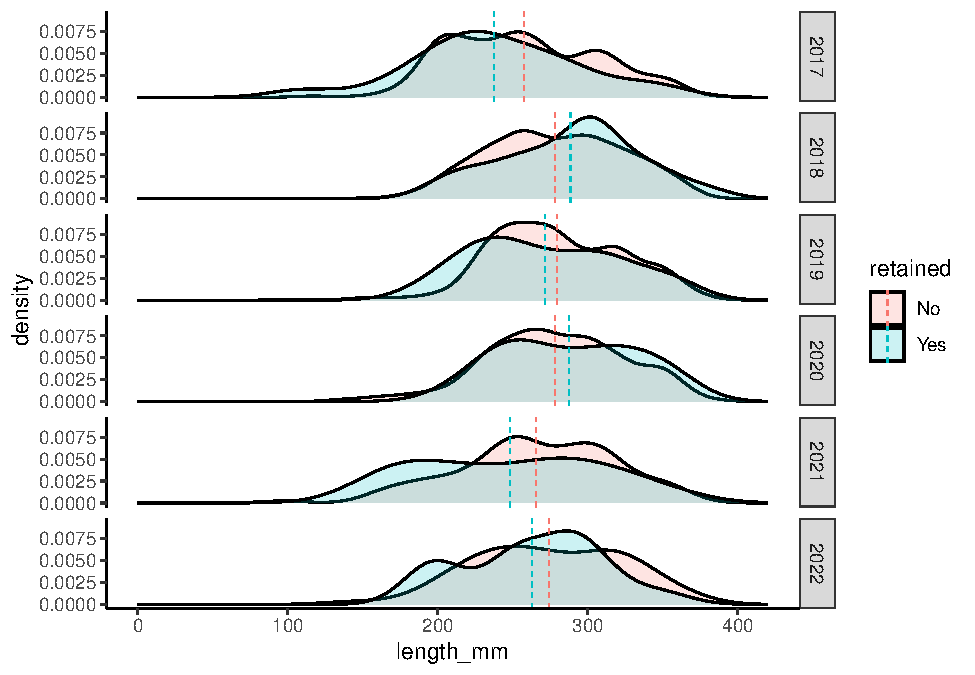
\includegraphics{CCRFP_species_otolith_summary_2023_files/figure-latex/unnamed-chunk-3-1.pdf}

\begin{longtable}[t]{lrr}
\caption{\label{tab:unnamed-chunk-4}Poly blue}\\
\toprule
year & No & Yes\\
\midrule
\endfirsthead
\caption[]{\label{tab:unnamed-chunk-4}Poly blue \textit{(continued)}}\\
\toprule
year & No & Yes\\
\midrule
\endhead

\endfoot
\bottomrule
\endlastfoot
\cellcolor{gray!6}{2017} & \cellcolor{gray!6}{2470} & \cellcolor{gray!6}{21}\\
2018 & 1881 & 26\\
\cellcolor{gray!6}{2019} & \cellcolor{gray!6}{934} & \cellcolor{gray!6}{43}\\
2020 & 1014 & 21\\
\cellcolor{gray!6}{2021} & \cellcolor{gray!6}{342} & \cellcolor{gray!6}{54}\\
\addlinespace
2022 & 80 & 17\\*
\end{longtable}

\end{document}
